\documentclass{fkssolpub}

\usepackage[czech]{babel}
\usepackage{fontspec}
\usepackage{fkssugar}
\usepackage{amsmath}
\usepackage{graphicx}

\author{Ondřej Sedláček}
\school{Gymnázium Oty Pavla} 
\series{2}
\problem{C} 

\renewcommand{\angle}{\sphericalangle}

\begin{document}

\begin{figure}
	\begin{center}
		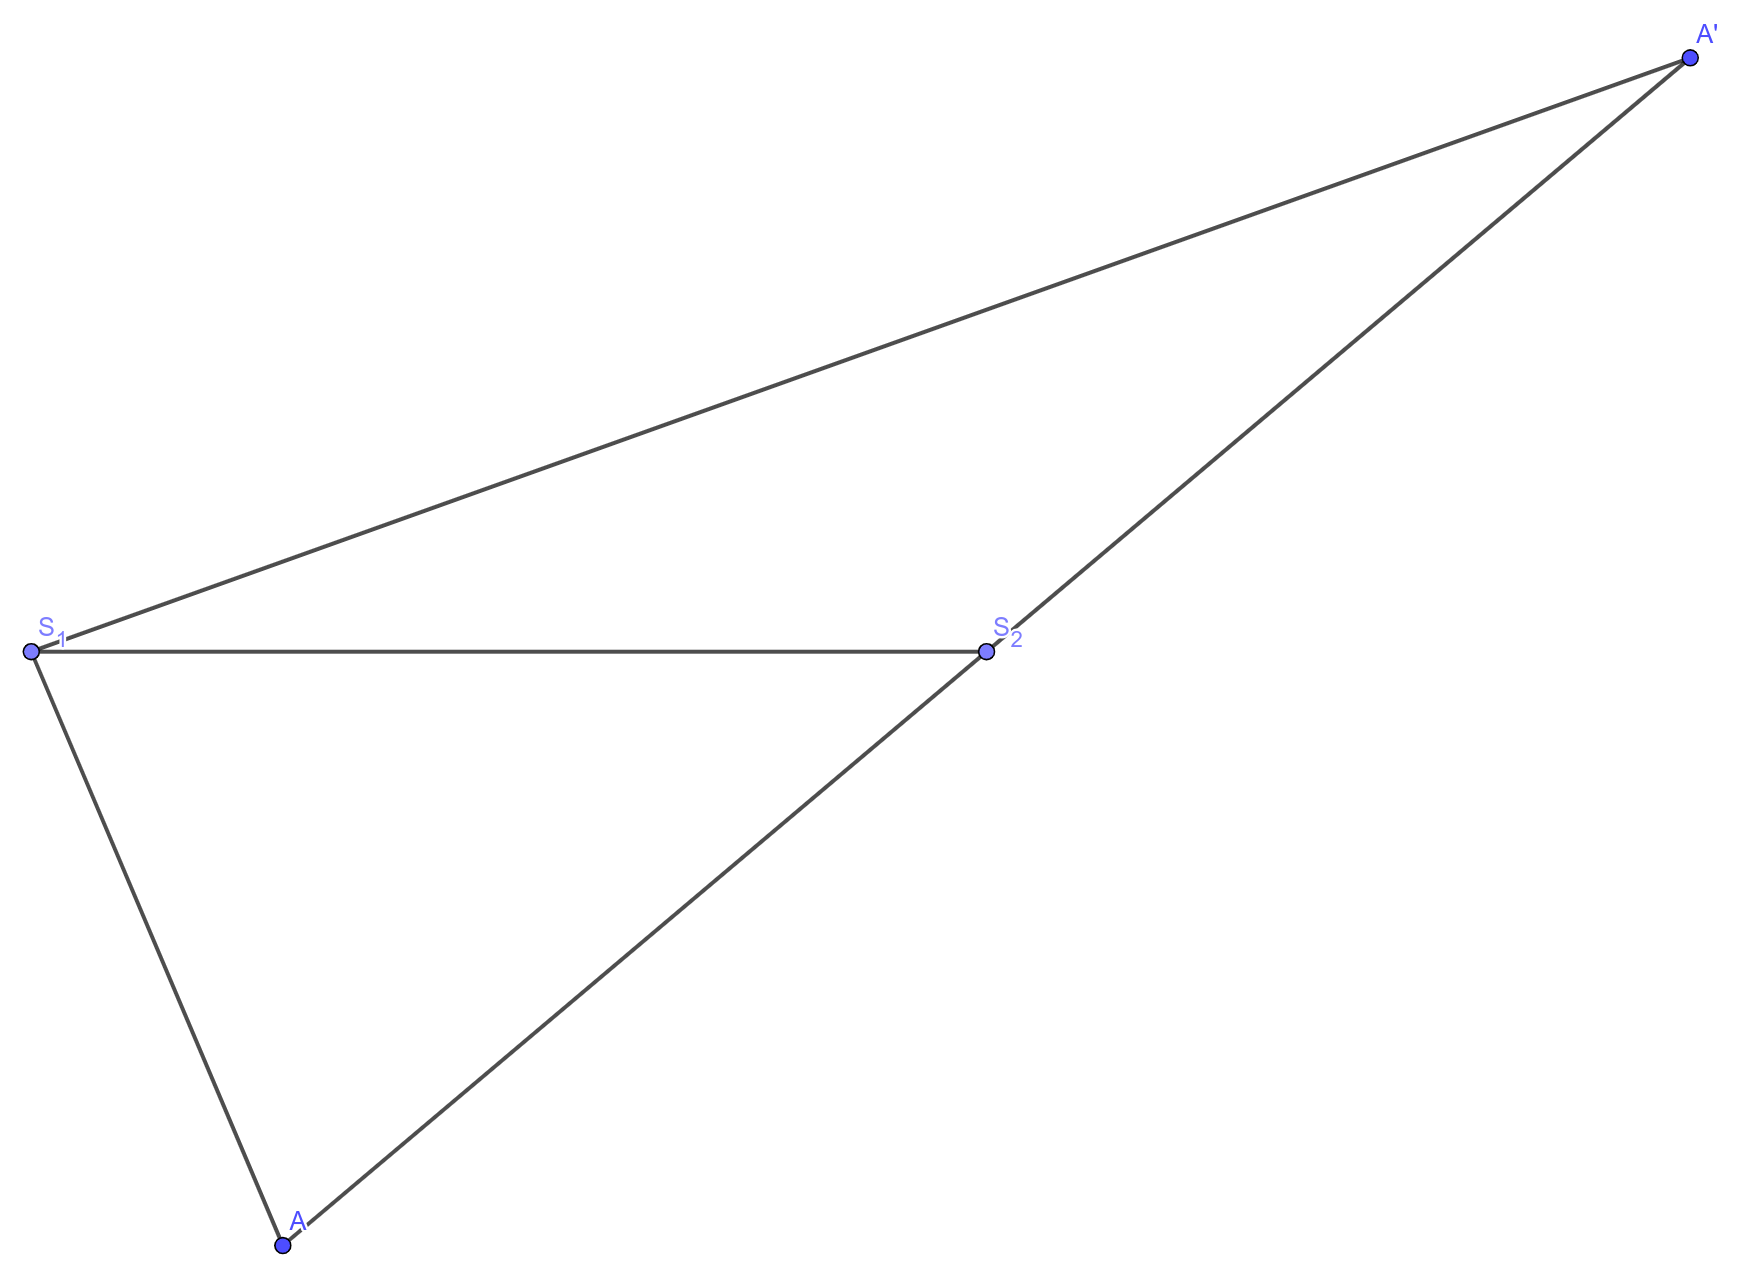
\includegraphics[width=0.95\textwidth]{C-fig}
	\end{center}
	\caption{Konstrukce toho, když zobrazíme bod přes vzdálenější střed}
	\label{fig:1}
\end{figure}

Nejprve dokážu, že pokud množina a její středy leží na přímce, tak nemůže být množina omezená. Nechť máme bod $A$ a dva středy $S_1$, $S_2$ (pokud je jich více, vybereme dva). Pak pokud $|AS_1| > |AS_2|$, pak pro obraz $A'$ přes střed $S_1$, který se nutně v této množině nachází, platí, že $|A' S_1| + |S_1 S_2| = |A'S_2| > |AS_1|$, tedy se obraz vzdálil od středů souměrnosti. Ale tento postup můžeme zopakovat pro každý obraz, který se bude pak vzdalovat do nekonečna. To je ale ve sporu s tím, že množina je omezená. Tím jsme ošetřili tento případ a můžeme dokázat případy, kdy vybrané středy a bod $A$ budou tvořit trojúhelník.

Pro tento důkaz jako první ukážu, že pokud nějaký bod $A$ zobrazíme přes vzdálenější střed souměrnosti $S_2$, pak pro obraz $A'$ bude platit $|S_1A| \leq |S_2 A| < |S_1A'|$.

Pokud $|S_1A| \leq |S_2 A|$, pak taky $|\angle AS_2 S_1| \leq |\angle S_2 S_1 A|$, a proto úhel $\angle AS_2 S_1$ je nutně ostrý. Tím pádem úhel $\angle S_1 S_2 A'$ je úhel tupý a tedy je nutně větší než úhly $\angle S_2 A' S_1$ a $\angle A'S_1 S_2$. Z toho tedy platí, že $|S_1 A'| > |S_2 A'|$, a protože $|S_2 A| = |S_2 A'|$, také platí $|S_1 A'| > |S_2 A|$. Tím jsme dokázali tvrzení výše.

Teď dokážeme sporem, že omezená množina nemůže mít více než jeden střed. Nechť bod $A$ je součástí této množiny a $S_1$, $S_2$ jsou dva ze středů souměrnosti této množiny. Pak když získáme obraz přes vzdálenější střed souměrnosti $A'$, který je nutně součástí této množiny, pak pomocí tvrzení dokázané výše ukážeme, že bod $A'$ bude vzdálenější od středů souměrnosti než bod $A$. Tento postup ale můžeme opakovat donekonečna a dostaneme vždy bod, který bude vzdálenější od středů souměrností. A to je spor s tím, že množina je omezená. Tím je tedy celý důkaz u konce.

\end{document}
